\documentclass[onlytextwidth, aspectratio=169]{beamer}
\usepackage[utf8]{inputenc}
\usepackage{microtype}
\usepackage{amsmath}
\usepackage{amssymb}
\usepackage[nomessages]{fp} %\FPeval{\var-name}{2*sin(pi/6)}
\usepackage{siunitx} %units in math. eg 20\milli\meter
\usepackage{yhmath} % for arcs, overparenth command
\usepackage{tikz} %graphics
\usetikzlibrary{quotes, angles, arrows, arrows.meta}
%\usepackage{graphicx} already loaded by beamer class
%consider setting \graphicspath{{images/}}
%\parskip ?? to avoid paragraph indent
\usepackage{multicol} %may not need this package, just columns environment
\usepackage{venndiagram}

\subtitle[BECA]{Bronx Early College Academy}
\author[Huson]{Christopher J. Huson PhD}

\setbeamertemplate{headline}{\vskip2mm 
  \, BECA / \insertshortauthor \, / \inserttitle
  \hfill 
  \insertsection
  }

%Tick mark commands
\newcommand\ticks{}
  \def\ticks{{Bar[scale=2]}-{Bar[scale=2]}}
\newcommand\paraticks{}
  \def\paraticks{{Straight Barb[reversed, scale=2]}-{Straight Barb[scale=2]}}

\title{Geometry Unit 6: Analytic Geometry}
\date{7 December 2022 - 13 January 2023}

\begin{document}
\frame{\titlepage}
\section[Outline]{}
\frame{\tableofcontents}

\section{6.1 Midpoint formula \hfill 8 December \,}
\begin{frame}{Learning Target: I can plot a midpoint on the plane}
  {HSG.GPE.B.6 Partition a line segment \hfill \alert{6.1 Thursday 8 December}}
  \begin{block}{Do Now}
    \begin{enumerate}
      \item Review your Jumprope grades
      \item Find the midpoint $M$ of $\overline{AB}$
    \end{enumerate}
    \begin{center}
      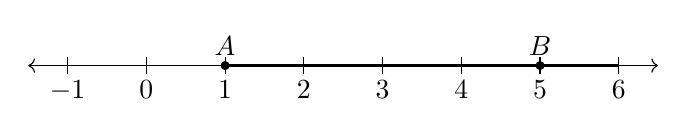
\begin{tikzpicture}
        \draw[<->] (-1.5,0)--(6.5,0);
        \foreach \x in {-1,...,6}
          \draw[shift={(\x,0)}] (0pt,-3pt)--(0pt,3pt) node[below=5pt]{$\x$};
        \draw[fill] (1,0) circle [radius=0.05] node[above]{$A$};
        \draw[fill] (5,0) circle [radius=0.05] node[above]{$B$};
        \draw[thick] (1,0)--(6,0);
      \end{tikzpicture}
    \end{center} 
  \end{block}
    Lesson: Midpoint and average, classwork practice \\
    Homework: Deltamath midpoint practice (optional extension)
\end{frame}

\begin{frame}{What do you know about the coordinate plane?}
    \begin{columns}
      \column{0.7\textwidth}
      \begin{description}
        \item[Coordinates] Values locating a point on a plane $(x,y)$
        \item[Axis] The two number lines, $x$ and $y$-axis
        \item[Origin] The center of the plane, $(0,0)$
        \item[Quadrant] The four quarters of the plane 
      \end{description}
      \column{0.3\textwidth}
      \begin{flushright}
        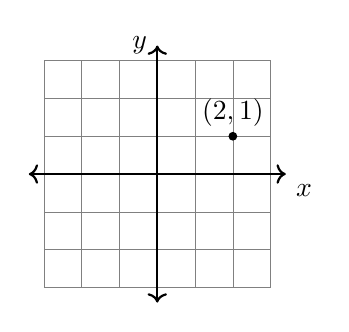
\begin{tikzpicture}[scale=.48]
          \draw [help lines] (-3,-3) grid (3,3);
          \draw [thick, <->] (-3.4,0) -- (3.4,0) node [below right] {$x$};
          \draw [thick, <->] (0,-3.4)--(0,3.4) node [left] {$y$};
          \draw [fill] (2,1) circle [radius=0.1] node[above] {$(2,1)$};
        \end{tikzpicture}
      \end{flushright}
    \end{columns} \vspace{0.5cm}
  \end{frame}

\begin{frame}{The midpoint formula}
  \begin{columns}
    \column{0.5\textwidth}
    Given $A(x_A,y_A)$, $B(x_B,y_B)$, midpoint $$\displaystyle M = \left(\frac{x_A+x_B}{2}, \frac{y_A+y_B}{2}\right)$$ \vspace{0.5cm}
    \column{0.5\textwidth}
    \begin{flushright}
      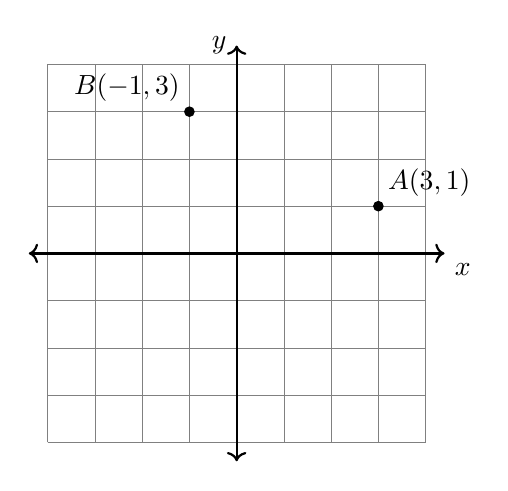
\begin{tikzpicture}[scale=0.6]
        \draw [help lines] (-4,-4) grid (4,4);
        \draw [thick, <->] (-4.4,0) -- (4.4,0) node [below right] {$x$};
        \draw [thick, <->] (0,-4.4)--(0,4.4) node [left] {$y$};
        \draw [fill] (3,1) circle [radius=0.1] node[above right] {$A(3,1)$};
        \draw [fill] (-1,3) circle [radius=0.1] node[above left] {$B(-1,3)$};
      \end{tikzpicture}
    \end{flushright}
  \end{columns} \vspace{0.5cm}
\end{frame}

\section{6.2 Slope-intercept form \hfill 9 December \,}
\begin{frame}{Learning Target: I can use slope-intercept form of linear equations}
  {8.F.A.3 Interpret $y=mx+b$ as a linear function, whose graph is a straight line \hfill \alert{6.2 Friday 9 December}}
  \begin{columns}
    \column{0.5\textwidth}
      Do Now: Find the midpoint $M$ of $\overline{AB}$ \\[1cm]
      Lesson: Slope, $y$-intercept, linear equations \\
      Homework: Deltamath graphing practice (optional extension)
    \column{0.5\textwidth}
    \begin{flushright}
      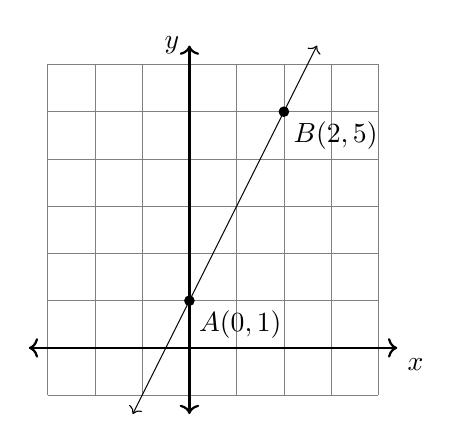
\begin{tikzpicture}[scale=0.6]
        \draw[help lines] (-3,-1) grid (4,6);
        \draw[thick, <->] (-3.4,0) -- (4.4,0) node [below right] {$x$};
        \draw[thick, <->] (0,-1.4)--(0,6.4) node [left] {$y$};
        \draw[<->,domain=-1.2:2.7] plot (\x, 2*\x+1) ;
        \draw [fill] (0,1) circle [radius=0.1] node[below right] {$A(0,1)$};
        \draw [fill] (2,5) circle [radius=0.1] node[below right] {$B(2,5)$};
      \end{tikzpicture}
    \end{flushright}
  \end{columns}
\end{frame}

\begin{frame}{Linear equations of the form $y=mx+b$}
  \begin{columns}
    \column{0.6\textwidth}
    \begin{description}
      \item[Linear] Straight, constant rate of change
      \item[Intercept] Where the line crosses the axis
      \item[$b$] $y$-intercept, point $(0,b)$ when $x=0$
      \item[Increasing] Going up. $y$ increases as $x$ increases
      \item[Decreasing] Going down. $y$ decreases as $x$ increases
      \item[$m$, slope] How steep the line is 
      $$m=\frac{rise}{run}=\frac{y_B-y_A}{x_B-x_A}$$
    \end{description}
    \column{0.4\textwidth}
    \begin{flushright}
      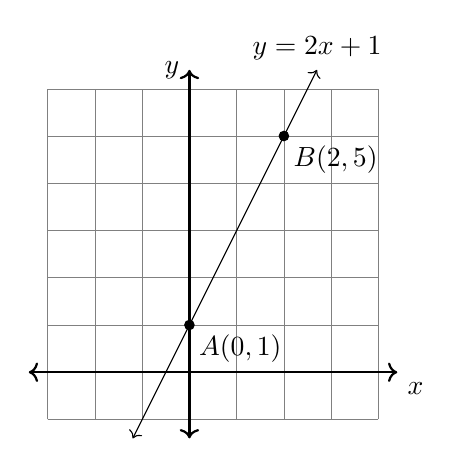
\begin{tikzpicture}[scale=0.6]
        \draw[help lines] (-3,-1) grid (4,6);
        \draw[thick, <->] (-3.4,0) -- (4.4,0) node [below right] {$x$};
        \draw[thick, <->] (0,-1.4)--(0,6.4) node [left] {$y$};
        \draw[<->,domain=-1.2:2.7] plot (\x, 2*\x+1) node[above]{$y=2x+1$};
        \draw [fill] (0,1) circle [radius=0.1] node[below right] {$A(0,1)$};
        \draw [fill] (2,5) circle [radius=0.1] node[below right] {$B(2,5)$};
      \end{tikzpicture}
    \end{flushright}
  \end{columns}
\end{frame}

\section{6.3 Functions, standard form \hfill 12 December \,}
\begin{frame}{Learning Target: I can use the standard form of linear equations}
  {8.F.A.3 Interpret $y=mx+b$ as a linear function, whose graph is a straight line \hfill \alert{6.3 Monday 12 December}}
  \begin{columns}
    \column{0.5\textwidth}
      Do Now: Find the equation of $\overleftrightarrow{AB}$ \\[1cm]
      Lesson: Function notation, vertical and horizontal slopes, the standard form of linear equations (GraspableMath practice) \\
      Homework: Handout problem set
    \column{0.5\textwidth}
    \begin{flushright}
      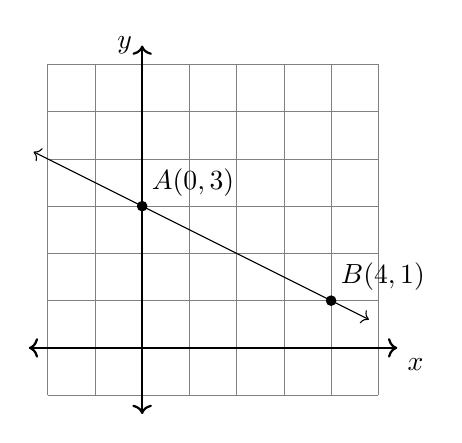
\begin{tikzpicture}[scale=0.6]
        \draw[help lines] (-2,-1) grid (5,6);
        \draw[thick, <->] (-2.4,0) -- (5.4,0) node [below right] {$x$};
        \draw[thick, <->] (0,-1.4)--(0,6.4) node [left] {$y$};
        \draw[<->,domain=-2.3:4.8] plot (\x, -0.5*\x+3) ;
        \draw[fill] (0,3) circle [radius=0.1] node[above right] {$A(0,3)$};
        \draw[fill] (4,1) circle [radius=0.1] node[above right] {$B(4,1)$};
      \end{tikzpicture}
    \end{flushright}
  \end{columns}
\end{frame}

\begin{frame}{Function notation, $f(x)=mx+b$}
  \begin{columns}
    \column{0.6\textwidth}
    \begin{description}
      \item[Function] $(x,y)$ pairs that satisfy a rule, $f(x)=y$
      \item[Horizontal] Slope is zero, $m=0$
      \item[Vertical] Slope is undefined, $m=\infty$
      \item[Domain] The set of $x$ values that are allowed
      \item[Range] The set of $y$ values that are allowed
      \item[Real numbers] The set of all numbers, $\mathbb{R}$
    \end{description}
    \column{0.4\textwidth}
    \begin{flushright}
      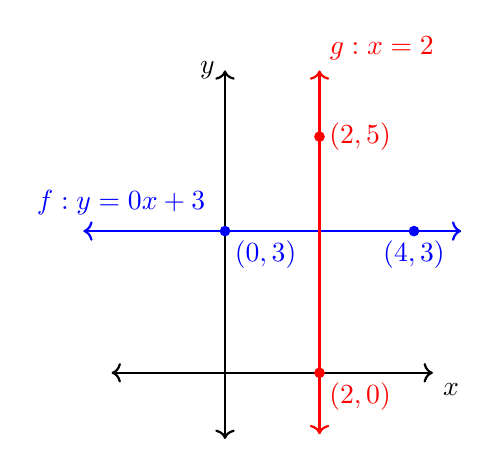
\begin{tikzpicture}[scale=0.6]
        \draw[thick, <->] (-2.4,0) -- (4.4,0) node [below right] {$x$};
        \draw[thick, <->] (0,-1.4)--(0,6.4) node [left] {$y$};
        \draw[thick, <->,domain=-3:5, color=blue] plot (\x, 3);
        \node at (-2.2,3.6)[color=blue]{$f: y=0x+3$};
        \draw[thick, <->, color=red] (2,-1.3)--(2,6.4) node [above right] {$g: x=2$};
        \draw[fill, blue] (0,3) circle [radius=0.1] node[below right] {$(0,3)$};
        \draw[fill, blue] (4,3) circle [radius=0.1] node[below] {$(4,3)$};
        \draw[fill, red] (2,0) circle [radius=0.1] node[below right] {$(2,0)$};
        \draw[fill, red] (2,5) circle [radius=0.1] node[right] {$(2,5)$};
      \end{tikzpicture}
    \end{flushright}
  \end{columns}
\end{frame}

\begin{frame}{Linear equations of the form $ax+by=c$}
    \begin{description}
      \item[Standard form] A linear equation written in the form $ax+by=c$
      \item[Calculator form] Casios and other calculators use the form $y=mx+b$
    \end{description} \vspace{1cm}
Convert from standard to $y$-intercept form. Example: 
  $$x+2y=6$$
\end{frame}

\section{6.4 Parallel and perpendicular slopes \hfill 13 December \,}
\begin{frame}{Learning Target: I can find parallel and perpendicular slopes}
  {HSG.GPE.B.5 The slope criteria for parallel and perpendicular lines \hfill \alert{6.4 Tuesday 13 December}}
  \begin{columns}
    \column{0.5\textwidth}
      Do Now: Find the equation of $\overleftrightarrow{AB}$ \\
      Challenge: find the $x$-intercept \\[1cm]
      Lesson: Parallel and perpendicular lines, negative reciprocals \\
      Homework: Deltamath problem set
    \column{0.5\textwidth}
    \begin{flushright}
      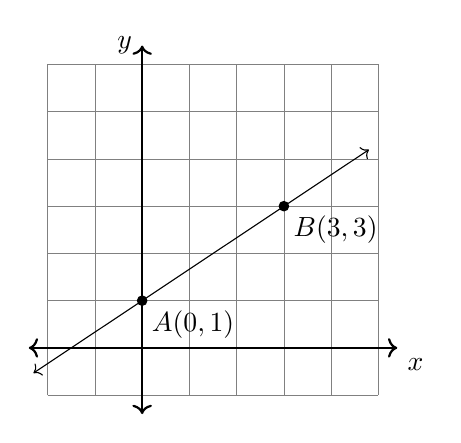
\begin{tikzpicture}[scale=0.6]
        \draw[help lines] (-2,-1) grid (5,6);
        \draw[thick, <->] (-2.4,0) -- (5.4,0) node [below right] {$x$};
        \draw[thick, <->] (0,-1.4)--(0,6.4) node [left] {$y$};
        \draw[<->,domain=-2.3:4.8] plot (\x, 0.666*\x+1) ;
        \draw[fill] (0,1) circle [radius=0.1] node[below right] {$A(0,1)$};
        \draw[fill] (3,3) circle [radius=0.1] node[below right] {$B(3,3)$};
      \end{tikzpicture}
    \end{flushright}
  \end{columns}
\end{frame}

\begin{frame}{Parallel lines have the same slope}
  \begin{columns}
    \column{0.5\textwidth}
    \begin{description}
      \item[Parallel] Lines in the same plane that never intersect
      \item[Skew] Lines that do not intersect and are not parallel
    \end{description} \bigskip
    Lines $k$ and $l$ are parallel if and only if $m_k=m_l$, if their slopes are equal.
    \column{0.5\textwidth}
    \begin{flushright}
      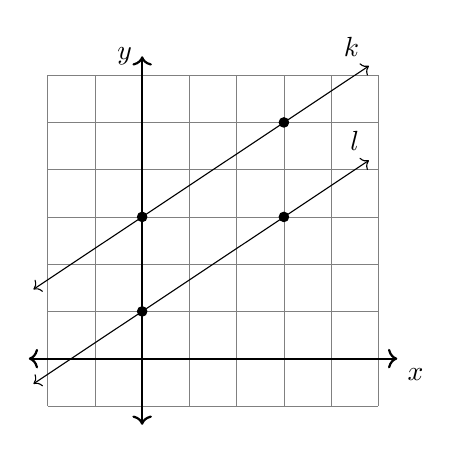
\begin{tikzpicture}[scale=0.6]
        \draw[help lines] (-2,-1) grid (5,6);
        \draw[thick, <->] (-2.4,0) -- (5.4,0) node [below right] {$x$};
        \draw[thick, <->] (0,-1.4)--(0,6.4) node [left] {$y$};
        \draw[<->,domain=-2.3:4.8] plot (\x, 0.666*\x+1) node[above left]{$l$};
        \draw[fill] (0,1) circle [radius=0.1];
        \draw[fill] (3,3) circle [radius=0.1];
        \draw[<->,domain=-2.3:4.8] plot (\x, 0.666*\x+3) node[above left]{$k$};
        \draw[fill] (0,3) circle [radius=0.1];
        \draw[fill] (3,5) circle [radius=0.1];
      \end{tikzpicture}
    \end{flushright}
  \end{columns}
\end{frame}

\begin{frame}{Perpendicular lines slopes' are negative reciprocals}
  \begin{columns}
    \column{0.55\textwidth}
    \begin{description}
      \item[Perpendicular] Lines that intersect at right angles
      \item[Reciprocals] Two numbers whose product is 1
      \item[Quarter turn] $90^\circ$ rotation, reversing the sign of the slope and the $x$ and $y$ coordinates
    \end{description} \bigskip
    Lines $k$ and $l$ are perpendicular if and only if $m_k \times m_l = -1$, if their slopes are negative reciprocals.
    \column{0.45\textwidth}
    \begin{flushright}
      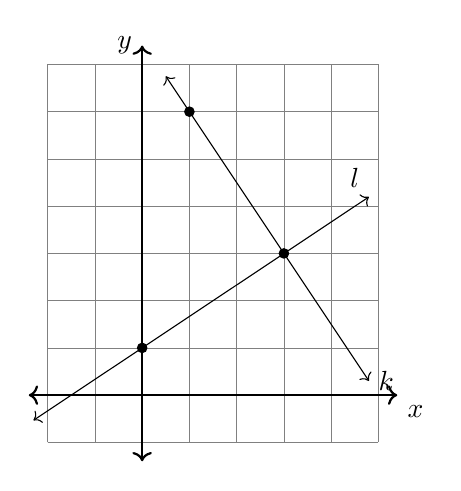
\begin{tikzpicture}[scale=0.6]
        \draw[help lines] (-2,-1) grid (5,7);
        \draw[thick, <->] (-2.4,0) -- (5.4,0) node [below right] {$x$};
        \draw[thick, <->] (0,-1.4)--(0,7.4) node [left] {$y$};
        \draw[<->,domain=-2.3:4.8] plot (\x, 0.666*\x+1) node[above left]{$l$};
        \draw[fill] (0,1) circle [radius=0.1];
        \draw[fill] (3,3) circle [radius=0.1];
        \draw[<->,domain=0.5:4.8] plot (\x, -1.5*\x+7.5) node[right]{$k$};
        \draw[fill] (1,6) circle [radius=0.1];
      \end{tikzpicture}
    \end{flushright}
  \end{columns}
\end{frame}

\section{6.5 Review linear equations \hfill 13 December \,}
\begin{frame}{Learning Target: I can graph linear equations}
  {8.F.A.3 Interpret $y=mx+b$ as a linear function, whose graph is a straight line \hfill \alert{6.5 Wednesday 14 December}}
  \begin{block}{Prequiz roundtable groupwork}
    Do Now: Organize and complete worksheets
    \begin{itemize}
      \item[6.5] Prequiz: Review slope-intercept form of linear equations
      \item[6.4] Classwork: Parallel and perpendicular slopes
      \item[6.3] Homework: Standard form
      \item[6.2] Classwork: Linear equations
      \item[6.1] Classwork: Midpoints
    \end{itemize}
      Lesson: Peer review of linear equations \\
      Homework: Study for quiz on Thursday \\
      Deltamath due Friday
  \end{block}
\end{frame}

\section{6.6 Quiz linear equations \hfill 16 December \,}
\begin{frame}{Quiz: Slope and linear equations \hfill \alert{6.6 Friday 16 December}}
  8.F.A.3 Interpret $y=mx+b$ as a linear function, whose graph is a straight line \\
  HSG.GPE.B.5 The slope criteria for parallel and perpendicular lines \\ \vspace{1cm}
  Do Now: Turn in worksheets (Deltamath due) \vspace{0.5cm}
  \begin{block}{Open notebook, calculator allowed}
  \end{block} \vspace{2cm}
\end{frame}

\section{6.7 Systems \hfill 3 January \,}
\begin{frame}{Learning Target: I can solve two equations in two variables}
  {HSG.REI.C.6 Solve systems of linear equations \hfill \alert{6.7 Tuesday 3 January}}
  \begin{columns}
    \column{0.5\textwidth}
      Do Now: Find the equations of $\overleftrightarrow{AC}$ and  $\overleftrightarrow{BC}$\\
      Are they perpendicular? \\[1cm]
      Lesson: Systems of equations, two intersecting lines \\
      Homework: Deltamath problem set
    \column{0.5\textwidth}
    \begin{flushright}
      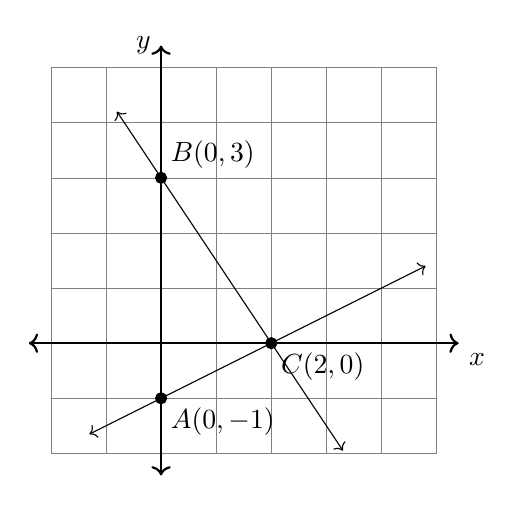
\begin{tikzpicture}[scale=0.7]
        \draw[help lines] (-2,-2) grid (5,5);
        \draw[thick, <->] (-2.4,0) -- (5.4,0) node [below right] {$x$};
        \draw[thick, <->] (0,-2.4)--(0,5.4) node [left] {$y$};
        \draw[<->,domain=-1.3:4.8] plot (\x, 0.5*\x-1);
        \draw[<->,domain=-0.8:3.3] plot (\x, -1.5*\x+3);
        \draw[fill] (0,-1) circle [radius=0.1] node[below right] {$A(0,-1)$};
        \draw[fill] (0,3) circle [radius=0.1] node[above right] {$B(0,3)$};
        \draw[fill] (2,0) circle [radius=0.1] node[below right] {$C(2,0)$};
      \end{tikzpicture}
    \end{flushright}
  \end{columns}
\end{frame}

\begin{frame}{Systems of equations}
  \begin{columns}
    \column{0.6\textwidth}
    \begin{align*}
      \overleftrightarrow{AC}: y &= + \frac{1}{2} x-1 \\
      \overleftrightarrow{BC}: y &= -\frac{3}{2} x+3
    \end{align*}
    Lines are not perpendicular: $\frac{1}{2} \times -\frac{3}{2} \ne -1$ (slopes are not negative reciprocals) \bigskip
    \begin{description}
      \item[Systems] Multiple equations with the same variables
      \item[Intersection] Point that satisfies both equations
      \item[Solution] Values $(x,y)$ that satisfy both equations
    \end{description} \bigskip
    \column{0.40\textwidth}
    \begin{flushright}
      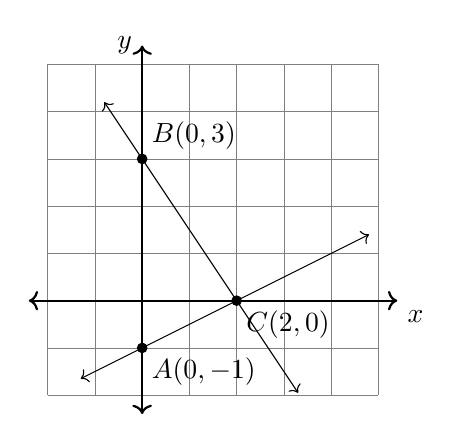
\begin{tikzpicture}[scale=0.6]
        \draw[help lines] (-2,-2) grid (5,5);
        \draw[thick, <->] (-2.4,0) -- (5.4,0) node [below right] {$x$};
        \draw[thick, <->] (0,-2.4)--(0,5.4) node [left] {$y$};
        \draw[<->,domain=-1.3:4.8] plot (\x, 0.5*\x-1);
        \draw[<->,domain=-0.8:3.3] plot (\x, -1.5*\x+3);
        \draw[fill] (0,-1) circle [radius=0.1] node[below right] {$A(0,-1)$};
        \draw[fill] (0,3) circle [radius=0.1] node[above right] {$B(0,3)$};
        \draw[fill] (2,0) circle [radius=0.1] node[below right] {$C(2,0)$};
      \end{tikzpicture}
    \end{flushright}
  \end{columns}
\end{frame}

\begin{frame}{\emph{T-chart} list of $(x,y)$ pairs satisfying a equation}
  \begin{center} 
    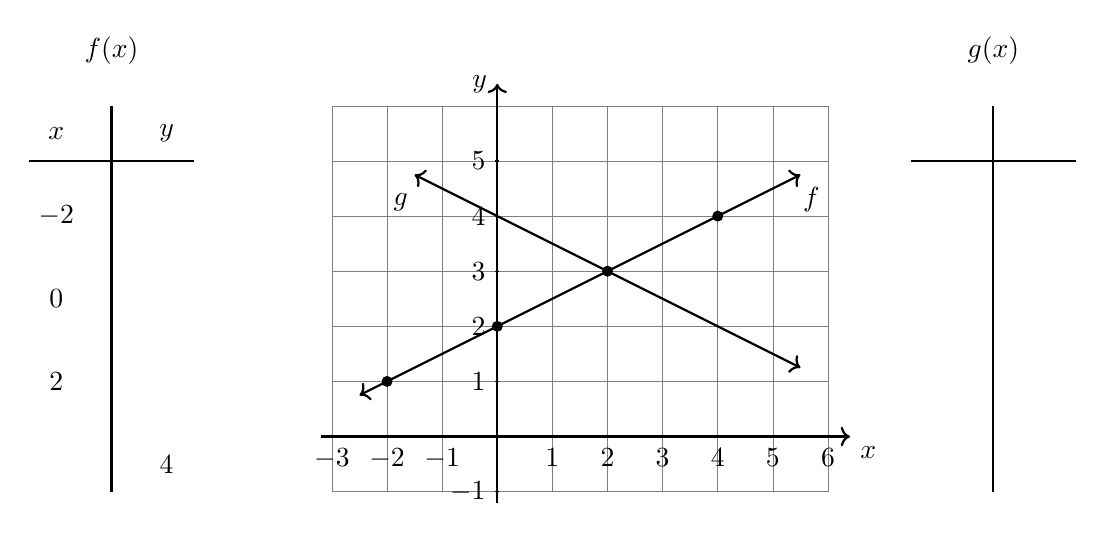
\begin{tikzpicture}[scale=0.7]
      \draw [help lines] (-3,-1) grid (6,6);
      \draw [thick, ->] (-3.2,0) -- (6.4,0) node [below right] {$x$};
      \draw [thick, ->] (0,-1.2)--(0,6.4) node [left] {$y$};
      \foreach \x in {-3,-2,-1,1,2,...,6} \draw (\x cm,1pt) -- (\x cm,-1pt) node[anchor=north] {$\x$};
      \foreach \y in {-1,1, 2, 3, 4, 5} \draw (1pt,\y cm) -- (-1pt,\y cm) node[anchor=east] {$\y$};
  
      \draw [thick, <->,samples=20,domain=-2.5:5.5] plot(\x,0.5*\x+2);
      \node at (5.7,4.3){$f$};
      \draw [thick, <->,samples=20,domain=-1.5:5.5] plot(\x,-0.5*\x+4);
      \node at (-1.75,4.25){$g$};
  
      \draw [thick] (-7,-1) -- (-7,6);
      \draw [thick] (-8.5,5) -- (-5.5,5);
      \node at (-7,7){$f(x)$};
      \node at (-8,5.5){$x$};
      \node at (-6,5.5){$y$};
      \draw [thick] (9,-1) -- (9,6);
      \draw [thick] (7.5,5) -- (10.5,5);
      \node at (9,7){$g(x)$};
      \node at (-8,4){$-2$}; 
      \node at (-8,2.5){$0$}; 
      \node at (-8,1){$2$}; 
      \node at (-6,-0.5){$4$};
      \fill (-2,1) circle[radius=0.1];
      \fill (0,2) circle[radius=0.1];
      \fill (2,3) circle[radius=0.1];
      \fill (4,4) circle[radius=0.1];
    \end{tikzpicture}
    \end{center}
\end{frame}

\begin{frame}{Solve the system for its solution, the intersection}
  {link to \href{https://activities.graspablemath.com/whiteboards/_f723f1056a7cd686}{Graspable Math} calculator}
  \begin{center} 
    \begin{tikzpicture}[scale=0.7]
      \draw [thick, ->] (-3.2,0) -- (6.4,0) node [below right] {$x$};
      \draw [thick, ->] (0,-1.2)--(0,7.4) node [left] {$y$};
      \foreach \x in {-4,-2,...,10} \draw (0.5*\x cm,1pt) -- (0.5*\x cm,-1pt) node[anchor=north] {$\x$};
      \foreach \y in {-2,0,...,12} \draw (1pt,0.5*\y cm) -- (-1pt,0.5*\y cm) node[anchor=east] {$\y$};
  
      \draw [thick] (-7,-1) -- (-7,6);
      \draw [thick] (-8.5,5) -- (-5.5,5);
      \node at (-7,7){$f(x)=\frac{2}{3}x+4$};
      \node at (-8,5.5){$x$};
      \node at (-6,5.5){$y$};
      \draw [thick] (9,-1) -- (9,6);
      \draw [thick] (7.5,5) -- (10.5,5);
      \node at (9,7){$g(x)=-\frac{1}{2}x+11$};
      \node at (8,5.5){$x$};
      \node at (10,5.5){$y$};
    \end{tikzpicture}
    \end{center}
\end{frame}

\begin{frame}{Solution: the intersection is {\color{red}$(6,8)$}}
  \begin{center} 
    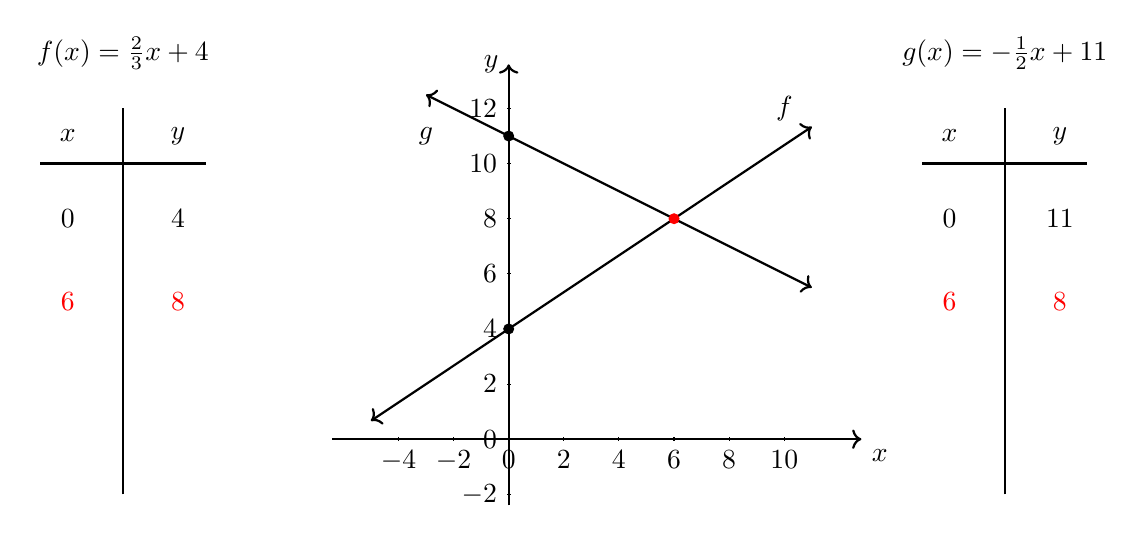
\begin{tikzpicture}[scale=0.7]
      \draw [thick, ->] (-3.2,0) -- (6.4,0) node [below right] {$x$};
      \draw [thick, ->] (0,-1.2)--(0,6.8) node [left] {$y$};
      \foreach \x in {-4,-2,...,10} \draw (0.5*\x cm,1pt) -- (0.5*\x cm,-1pt) node[anchor=north] {$\x$};
      \foreach \y in {-2,0,...,12} \draw (1pt,0.5*\y cm) -- (-1pt,0.5*\y cm) node[anchor=east] {$\y$};
  
      \draw [thick, <->,samples=20,domain=-2.5:5.5] plot(\x,0.667*\x+2);
      \node at (5,6){$f$};
      \draw [thick, <->,samples=20,domain=-1.5:5.5] plot(\x,-0.5*\x+5.5);
      \node at (-1.5,5.5){$g$};
  
      \draw [thick] (-7,-1) -- (-7,6);
      \draw [thick] (-8.5,5) -- (-5.5,5);
      \node at (-7,7){$f(x)=\frac{2}{3}x+4$};
      \node at (-8,5.5){$x$};
      \node at (-6,5.5){$y$};
      \node at (-8,4){$0$}; 
      \node at (-6,4){$4$};
      \node[color=red] at (-8,2.5){$6$}; 
      \node[color=red] at (-6,2.5){$8$}; 

      \draw [thick] (9,-1) -- (9,6);
      \draw [thick] (7.5,5) -- (10.5,5);
      \node at (9,7){$g(x)=-\frac{1}{2}x+11$};
      \node at (8,5.5){$x$};
      \node at (10,5.5){$y$};
      \node at (8,4){$0$}; 
      \node at (10,4){$11$};
      \node[color=red] at (8,2.5){$6$}; 
      \node[color=red] at (10,2.5){$8$}; 

      \fill (0,5.5) circle[radius=0.1];
      \fill (0,2) circle[radius=0.1];
      \fill[color=red] (3,4) circle[radius=0.1];
    \end{tikzpicture}
    \end{center}
\end{frame}

\section{6.8 Systems word problems \hfill 4 January \,}
\begin{frame}{Learning Target: I can solve linear systems in context}
  {HSG.REI.C.6 Solve systems of linear equations \hfill \alert{6.8 Wednesday 4 January}}
  Do Now:
  \begin{itemize}
    \item Laptop check: Raise your hand if your laptop has a 75+\% charge.
    \item Notebook check: find these formulas in your notebook \medskip
    \begin{enumerate}
      \item Slopes are perpendicular when $m \times m_\perp = -1$ \bigskip
      \item Distance $d = \sqrt{(x_2 - x_1)^2 + (y_2 - y_1)^2}$ \bigskip
      \item Midpoint $\displaystyle M = \bigl( \frac{x_1+x_2}{2}, \frac{y_1+y_2}{2} \bigr)$
    \end{enumerate}
  \end{itemize}
  Lesson: Solving word problems with systems of equations (Deltamath)
\end{frame}

\section{6.9 Word problems, quiz \hfill 6 January \,}
\begin{frame}{Learning Target: I can solve linear systems in context}
  {HSG.REI.C.6 Solve systems of linear equations \hfill \alert{6.9 Friday 6 January}}
  Do Now: Write two equations that model the following situation
  \begin{itemize}
    \item The total of two values is 10
    \item Twice one value plus five times the other totals 26. \medskip
  \end{itemize}
  Lesson: Solving word problems with systems of equations
  Assessment: Pop Quiz 6.9 Graphing Systems of Equations
\end{frame}

\begin{frame}{Solution: Graphing a system of equations to solve a word problem}
  \begin{columns}
    \column{0.4\textwidth}
    The total of two values is 10 \\
    Twice one value plus five times the other totals 26.
    \begin{align*}
      x+y=10 \\
      2x+5y=26
    \end{align*}
    Solution $x=8, y=2$ \par \medskip
    Check:
    \begin{align*}
      (8)+(2)=10  \checkmark \\
      2(8)+5(2)=26 \\
      16+10=26 \checkmark
    \end{align*}
    \column{0.6\textwidth}
    \begin{flushright}
      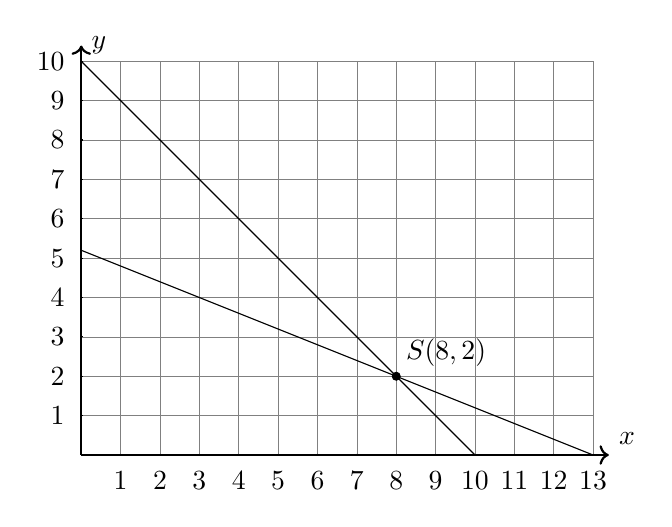
\begin{tikzpicture}[scale=0.5]
        \draw[help lines] (0,0) grid (13,10);
        \draw[thick, ->] (0,0) -- (13.4,0) node [above right] {$x$};
        \draw[thick, ->] (0,0)--(0,10.4) node [right] {$y$};
        \foreach \x in {1,2,...,13} \draw (\x cm,1pt) -- (\x cm,-1pt) node[below=2pt] {$\x$};
        \foreach \y in {1, 2, ...,10} \draw (1pt,\y cm) -- (-1pt,\y cm) node[left=2pt] {$\y$};
        \draw[domain=0:10] plot (\x, 10-\x);
        \draw[domain=0:13] plot (\x, -0.4*\x+5.2);
        \draw[fill] (8,2) circle [radius=0.1] node[above right] {$S(8,2)$};
      \end{tikzpicture}
    \end{flushright}
  \end{columns}
\end{frame}

\section{6.10 Quiz review, midpoint application \hfill 9 January \,}
\begin{frame}{Learning Target: I can apply the midpoint formula}
  {8.F.A.3 Interpret $y=mx+b$ as a linear function, whose graph is a straight line \hfill \alert{6.10 Monday 9 January}}
  \begin{columns}
    \column{0.5\textwidth}
      Do Now: Find the equation of $\overleftrightarrow{AB}$ \\[1cm]
      Lesson: Quiz review of linear equations, midpoint formula, distance calculation \\
      Homework: Deltamath practice problem set
    \column{0.5\textwidth}
    \begin{flushright}
      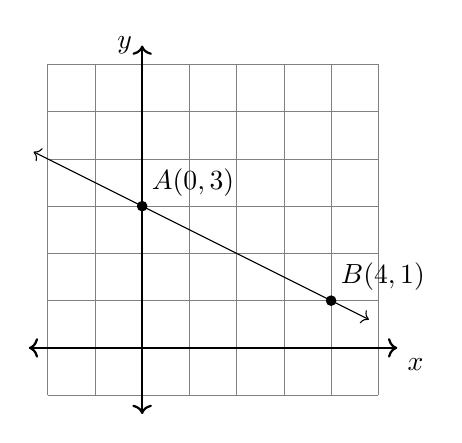
\begin{tikzpicture}[scale=0.6]
        \draw[help lines] (-2,-1) grid (5,6);
        \draw[thick, <->] (-2.4,0) -- (5.4,0) node [below right] {$x$};
        \draw[thick, <->] (0,-1.4)--(0,6.4) node [left] {$y$};
        \draw[<->,domain=-2.3:4.8] plot (\x, -0.5*\x+3) ;
        \draw[fill] (0,3) circle [radius=0.1] node[above right] {$A(0,3)$};
        \draw[fill] (4,1) circle [radius=0.1] node[above right] {$B(4,1)$};
      \end{tikzpicture}
    \end{flushright}
  \end{columns}
\end{frame}

\section{6.11 Quiz review, midpoint application \hfill 10 January \,}
\begin{frame}{Learning Target: I can use the point-slope form of linear equations}
  {HSG.GPE.B.6 Partition a line segment \hfill \alert{6.11 Tuesday 10 January}}
  \begin{columns}
    \column{0.5\textwidth}
      Do Now: Find the equation of the line through $P(3,4)$ with slope $m=\frac{2}{3}$ \\[1cm]
      Lesson: Point-slope form \\
      Homework: Deltamath practice problem set
      Test Friday
    \column{0.5\textwidth}
    \begin{flushright}
      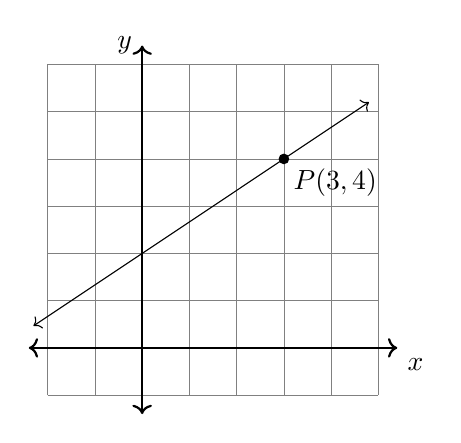
\begin{tikzpicture}[scale=0.6]
        \draw[help lines] (-2,-1) grid (5,6);
        \draw[thick, <->] (-2.4,0) -- (5.4,0) node [below right] {$x$};
        \draw[thick, <->] (0,-1.4)--(0,6.4) node [left] {$y$};
        \draw[<->,domain=-2.3:4.8] plot (\x, 0.667*\x+2) ;
        \draw[fill] (3,4) circle [radius=0.1] node[below right] {$P(3,4)$};
      \end{tikzpicture}
    \end{flushright}
  \end{columns}
\end{frame}

\begin{frame}{Point-slope form}
  A line through $P(x_0,y_0)$ with slope $m$ has equation $y-y_0=m(x-x_0)$
  \begin{columns}
    \column{0.5\textwidth}
      \begin{align*}
        y-4=\frac{2}{3}(x-3) \\
        y-4=\frac{2}{3}x-2 \\
        y=\frac{2}{3}x+2
      \end{align*}
      \begin{description}
        \item[Point-slope] $y-y_0=m(x-x_0)$
        \item[Standard form] $ax+by=c$
        \item[Slope-intercept] $y=mx+b$
      \end{description} \bigskip
    \column{0.5\textwidth}
      \begin{flushright}
      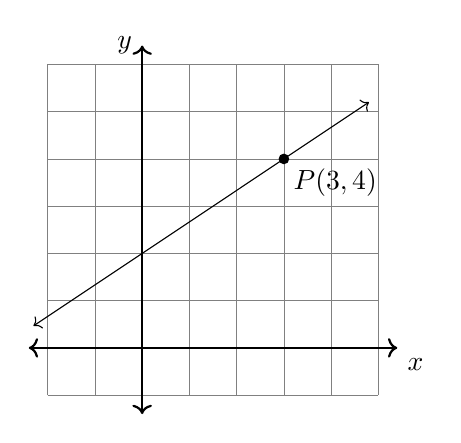
\begin{tikzpicture}[scale=0.6]
        \draw[help lines] (-2,-1) grid (5,6);
        \draw[thick, <->] (-2.4,0) -- (5.4,0) node [below right] {$x$};
        \draw[thick, <->] (0,-1.4)--(0,6.4) node [left] {$y$};
        \draw[<->,domain=-2.3:4.8] plot (\x, 0.667*\x+2) ;
        \draw[fill] (3,4) circle [radius=0.1] node[below right] {$P(3,4)$};
      \end{tikzpicture}
      \end{flushright}
  \end{columns}
\end{frame}

\section{6.12 Peer review \hfill 12 January \,}
\begin{frame}{Learning Target: I can use the point-slope form of linear equations}
  {HSG.GPE.B.6 Partition a line segment \hfill \alert{6.11 Thursday 12 January}}
  Exam review (open notebook), Deltamath and problem sets due Friday
  \begin{enumerate}
    \item 6.6 Quiz: Slope-intercept form of linear equations
    \item 6.7 Systems of linear equations
    \item 6.9 Classwork: Applications of systems of linear equations
    \item 6.9 Pop Quiz: Slope-intercept
    \item 6.10 Corrections: Slope-intercept
    \item 6.11 Classwork: Point-slope form
  \end{enumerate}
\end{frame}

\begin{frame}{Reminder that BECA's High School Uniform is as follows:}
  {Uniform should be worn at all times throughout the school day.}
  
  \begin{itemize}
    \item Navy Blue Polo with a School Logo
    \item Navy Blue Pullover with BECA on it
    \item Khaki bottoms
    \item Closed shoes
  \end{itemize} \vspace{0.5cm}
  All outerwear that is not stated above must go in your assigned lockers. Lockers should be used during the start and end of the day. \\[0.5cm]
  Failure to wear uniform will lead to removal from activities such as CAP, PSAL Sports, clubs, and incentives.
\end{frame}

\end{document}